\documentclass[twocolumn, 10pt]{article}
\setlength\textwidth{6.875in}
\setlength\textheight{8.875in}
% set both margins to 2.5 pc
\setlength{\oddsidemargin}{-0.1875in}% 1 - (8.5 - 6.875)/2
\setlength{\evensidemargin}{-0.1875in}
\setlength{\marginparwidth}{0pc}
\setlength{\marginparsep}{0pc}%
\setlength{\topmargin}{0in} \setlength{\headheight}{0pt}
\setlength{\headsep}{0pt}
\setlength{\footskip}{37pt}%
%\setlength{\columnsep}{0.3125in}
%\setlength{\columnwidth}{3.28125in}% (6.875 - 0.3125)/2 = 3.28125in
\setlength{\parindent}{1pc}
\newcommand{\myMargin}{1.00in}
\usepackage[top=\myMargin, left=\myMargin, right=\myMargin, bottom=\myMargin, nohead]{geometry}
\usepackage{epsfig,graphicx}
\usepackage{palatino}
\usepackage{fancybox}
\usepackage{hyperref}
\usepackage[procnames]{listings}

% "define" Stanza
\usepackage[T1]{fontenc}  
\usepackage[scaled=0.82]{beramono}  
\usepackage{microtype} 

\sbox0{\small\ttfamily A}
\edef\mybasewidth{\the\wd0 }

\lstdefinelanguage{stanza}{
  morekeywords={circuit, defclass,defmodule,defbundle,definterface,defpackage,defn,%
    do,else,public,false,finally,%
    for,if,import,inherit,inst,match,%
    map,new,node,object,override,package,%
    super,this,throw,true,try,%
    type,val,var,when,while%,
    % yield,UInt,Bool,Bits,SInt
    },
  sensitive=true,
  morecomment=[l]{;;},
  morestring=[b]",
  morestring=[b]',
  morestring=[b]"""
}

\usepackage{color}
\definecolor{dkgreen}{rgb}{0,0.6,0}
\definecolor{gray}{rgb}{0.5,0.5,0.5}
\definecolor{mauve}{rgb}{0.58,0,0.82}

% Default settings for code listings
\lstset{frame=tb,
  language=stanza,
  aboveskip=3mm,
  belowskip=3mm,
  showstringspaces=false,
  columns=fixed, % basewidth=\mybasewidth,
  basicstyle={\small\ttfamily},
  numbers=none,
  numberstyle=\footnotesize\color{gray},
  % identifierstyle=\color{red},
  keywordstyle=\color{blue},
  commentstyle=\color{dkgreen},
  stringstyle=\color{mauve},
  frame=single,
  breaklines=true,
  breakatwhitespace=true,
  procnamekeys={input,output,wire, mem, reg, node, defn, val, var, defclass, definterface, defbundle, defmodule, defpackage},
  procnamestyle=\ttfamily\color{red},
  tabsize=2
}

\lstnewenvironment{stanza}[1][]
{\lstset{language=stanza,#1}}
{}

% "define" Stanza
\usepackage[T1]{fontenc}  
\usepackage[scaled=0.82]{beramono}  
\usepackage{microtype} 

\sbox0{\small\ttfamily A}
\edef\mybasewidth{\the\wd0 }

\lstdefinelanguage{stanza}{
  morekeywords={circuit, defclass,defmodule,defbundle,definterface,defpackage,defn,%
    do,else,public,false,finally,%
    for,if,import,inherit,input,inst,match,%
    map,mem,new,node,object,override,output,package,%
    reg,super,this,throw,true,try,%
    type,val,var,when,while,wire%,%
    % yield,UInt,Bool,Bits,SInt
    },
  sensitive=true,
  morecomment=[l]{;;},
  morestring=[b]",
  morestring=[b]',
  morestring=[b]"""
}

\usepackage{color}
\definecolor{dkgreen}{rgb}{0,0.6,0}
\definecolor{gray}{rgb}{0.5,0.5,0.5}
\definecolor{mauve}{rgb}{0.58,0,0.82}

% Default settings for code listings
\lstset{frame=tb,
  language=stanza,
  aboveskip=3mm,
  belowskip=3mm,
  showstringspaces=false,
  columns=fixed, % basewidth=\mybasewidth,
  basicstyle={\small\ttfamily},
  numbers=none,
  numberstyle=\footnotesize\color{gray},
  % identifierstyle=\color{red},
  keywordstyle=\color{blue},
  commentstyle=\color{dkgreen},
  stringstyle=\color{mauve},
  frame=single,
  breaklines=true,
  breakatwhitespace=true,
  procnamekeys={input,output,wire, mem, reg, node, defn, val, var, defclass, definterface, defbundle, defmodule, defpackage},
  procnamestyle=\ttfamily\color{red},
  tabsize=2
}




\lstset{basicstyle={\footnotesize\ttfamily}}

\newenvironment{commentary}
{ \vspace{-0.1in}
  \begin{quotation}
  \noindent
  \small \em
  \rule{\linewidth}{1pt}\\
}
{
  \end{quotation}
}

\title{Getting Started - Tutorial 02: Basic Types and Operations}
\author{Jonathan Bachrach, Vincent Lee \\
EECS Department, UC Berkeley\\
{\tt  \{jrb\}@eecs.berkeley.edu}
}
\date{\today}

\newenvironment{example}{\VerbatimEnvironment\begin{footnotesize}\begin{Verbatim}}{\end{Verbatim}\end{footnotesize}}
\newcommand{\kode}[1]{\begin{footnotesize}{\tt #1}\end{footnotesize}}

\def\code#1{{\tt #1}}

\def\note#1{\noindent{\bf [Note: #1]}}
%\def\note#1{}

\begin{document}
\maketitle{}

% Bits has been deprecated and therefore section has been removed from this document. Older commits may have Bits section somewhere.

\section{Chipper Assignments and Reassignments}

Wires are introduced using ports and \verb+wire+ definitions.
\verb+wire+ definitions allow either an initial top-level value using \verb+:=+ or a final assignment with the \verb+=+ syntax.
On every subsequent reassignment to the wire, we must use a \verb+:=+ when reassigning the value.

Since we are constructing a digital circuit, the notion of reassignment does not make much sense since connections between circuit nodes only need to be specified once. However, there are some cases when we will need to perform reassignment to a wire in Chipper since it is compiled sequentially unlike Verilog. Thus it may be necessary to perform reassignment when a value or connection is not known until later in the Chipper source. 

A simple example of when reassignment is necessary is in the construction of the top level I/O for your module; the values of the output are not immediately known at the time of declaration.

Consider the simple \verb+FullAdder+ circuit from previous tutorial that determines the sum \verb+sum+ and carry out \verb+cout+ given two values \verb+a+ and \verb+b+, and a carry in \verb+cin+.

\begin{stanza}
defmodule FullAdder :
  input a:     UInt<1>
  input b:     UInt<1>
  input cin:   UInt<1>
  output sum:  UInt<1>
  output cout: UInt<1>

  wire a_xor_b = a ^ b
  wire a_and_b = a & b
  sum  := a_xor_b ^ cin
  cout := a_and_b | (b & cin) | (a & cin)
\end{stanza}

In this example we make sure to use the \verb+:=+ reassignment for the \verb+sum+ and \verb+cout+ output values because we only know what they're values are later in the code and not at the time of port definition. All other wires in this example use the \verb+=+ assignment operator since their values are known at definition time. 

In general, the rule of thumb is to use the reassignment operator \verb+:=+ if the value already has been assigned by the \verb+=+ operator, otherwise the \verb+=+ operator should be used. Note that if you do not use the \verb+=+ or \verb+:=+ operators correctly you will get an error when you try and compile your design.

\section{The Chipper UInt Class}

In the previous examples we have been using the \verb+UInt+ type which is an unsigned integer as the type for all of our values. For many of the basic computations in Chipper the \verb+UInt+ class is sufficient.\footnote{The {\tt UInt} class definition for Chipper can be found in the chipper/src folder in the compiler source repository, not the chipper-tutorial. You can obtain the Chipper source by cloning {\tt https://github.com/ucb-bar/chipper.git}} The following example shows some of the commonly used \verb+UInt+ operations in the context of a simple \verb+ALU+\footnote{We ignore overflow and underflow in this example.}:

\begin{stanza}
class BasicALU extends Module {
  input  a      : UInt<4>
  input  b      : UInt<4>
  input  opcode : UInt<4>
  output output : UInt<4>

  output := UInt(0) 
  when opcode === UInt(0) :
    output := a                   ;; pass A
  else: when opcode === UInt(1)
    output := b                   ;; pass B
  else: when opcode === UInt(2)
    output := a + UInt(1)         ;; inc A by 1
  else: when opcode === UInt(3)
    output := a - UInt(1)         ;; inc B by 1
  else: when opcode === UInt(4)
    output := a + UInt(4)         ;; inc A by 4
  else: when opcode === UInt(5)
    output := a - UInt(4)         ;; dec A by 4
  else: when opcode === UInt(6)
    output := a + b               ;; add A and B
  else: when opcode === UInt(7)
    output := a - b               ;; sub B from A
  else: when opcode === UInt(8)
    output := (a < b)             ;; set on A < B
  else: 
    output := (a === b)           ;; set on A == B
\end{stanza}

You will notice that there are multiple reassignments to \verb+output+ inside a \verb+when+ block which indicates that the value of \verb+output+ can take many different values depending on the \verb+opcode+ in this example. Also notice that in order to specify constants to add to our operands, we must also specify them as a \verb+UInt+ type as \verb+UInt+ operations on different type operands is not allowed.

\begin{stanza}
;; Specify that 1 is a UInt type
output := a + UInt(1) 
\end{stanza}

A list of commonly used \verb+UInt+ operations is given in the table below:

\begin{center}
\begin{tabular}{| l | l | l | }
\hline
{\bf Operand} & {\bf Operation} & {\bf Output Type} \\ \hline
+ & Add & UInt  \\ \hline
- & Subtract & UInt  \\ \hline
$\ast$ & Multiply & UInt \\ \hline
/ & UInt Divide & UInt \\ \hline
% & Modulo & UInt \\ \hline
\~\ & Bitwise Negation & UInt \\ \hline
\^\ & Bitwise XOR & UInt\\ \hline
\& & Bitwise AND & UInt \\ \hline
 | & Bitwise OR & Bool \\ \hline
=== & Equal & Bool \\ \hline
!= & Not Equal & Bool \\ \hline
> & Greater & Bool \\ \hline
< & Less & Bool \\ \hline
>= & Greater or Equal & Bool \\ \hline
<= & Less or Equal & Bool \\ \hline
\end{tabular}
\end{center}

% Notice that the comparisons for the UInt type give you a Bool type back. In order to be able to assign the output of a comparison to a UInt type, we will need to cast the Bool to a UInt before the assignment. This is shown in the \verb+BasicALU+ example in the \verb+.otherwise+ block:
% 
% \begin{stanza}
% io.output :=  (io.a === io.b).toUInt() ;; set on A == B
% \end{stanza}
% 
% If we you do not cast the resulting Bool to a UInt the Chipper compiler will return an error.

\subsection{Bit Extraction}

The \verb+UInt+ class allows you to extract bits based on their index of their representation. Given an \verb+n+ bit wide value \verb+value+ we can extract the bits \verb+x+ through \verb+y+ (n > x > y >= 0) by simply doing the following:

\begin{stanza}
;; extracts the x through y bits of value
wire x_to_y = value[x, y]
\end{stanza}

Note that the higher index is specified first in the argument list when extraction the bits. Also notice that the bits in the \verb+UInt+ are zero indexed so the highest bit that can be extracted from an \verb+n+ bit wide value is \verb+n-1+.

If you just want to extract a single bit from the value, say bit \verb+x+ we simply need to specify a single index instead as follows:
\begin{stanza}
;; extract the x-th bit from value
val x_of_value = value[x]
\end{stanza}

A more concrete example of bit extraction in action is shown below. In this example, based on the value of the offset, we would like to select a byte from a word which is a common operation when loading a byte from word addressed memories:

\begin{stanza}
defmodule ByteSelector :
  input  in     : UInt<32>
  input  offset : UInt<2>
  output out    : UInt<8>

  out := UInt<8>(0)
  when offset === UInt(0) :
    out := in[7,0]   ;; pull out lowest byte
  else : when offset === UInt(1) :
    out := in[15,8]  ;; pull out second byte
  else : when offset === UInt(2) :
    out := in[23,16] ;; pull out third byte
  else :
    out := in[31,24] ;; pull out highest byte
\end{stanza}

\subsection{Bit Concatenation}

Chipper also allows you to easily concatenate bits together using \verb+cat+. Suppose you have a data bus that you would like to drive with two seperate words \verb+A+ and \verb+B+. In order to concatenate these two values together we simply say:

\begin{stanza}
wire A : UInt<32>
wire B : UInt<32>
wire bus = cat(A, B) ;; concatenate A and B
\end{stanza}

Again, the first argument to \verb+cat+ will be placed in the high part while the second argument gets the low part of \verb+bus+. Thus for this example bits 0 to 31 of \verb+bus+ correspond to \verb+B+, while bits 32 to 63 correspond to \verb+A+. 

\subsection{\problem{LFSR16}}

In this assignment, write the \verb+LFSR16+ circuit as shown below:

\begin{center}
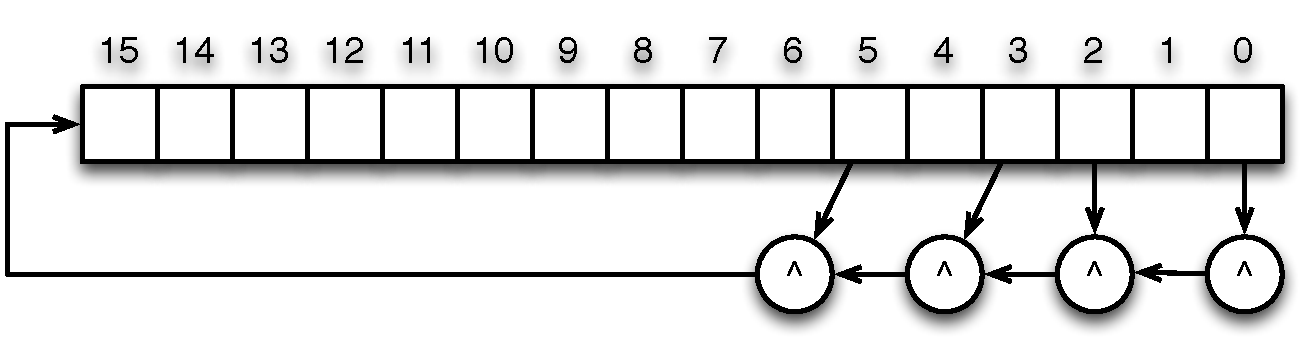
\includegraphics[width=0.9\columnwidth]{../bootcamp/figs/LFSR16.pdf}
\end{center}

\noindent
by filling in the following module:

\begin{stanza}
defmodule LFSR16 :
  input  inc : Bool
  output out : UInt<16>
  ;; ...
  out := UInt(0)
\end{stanza}

\noindent
found in \verb+$TUT_DIR/problems/LFSR16.stanza+.
Make sure to define and initialize an internal register to one and 
update it when \verb+inc+ is asserted.
Use bit concatentation and bit extraction 
in conjunction with the xor operator \verb+^+.  Run 

\begin{bash}
make LFSR16.out
\end{bash}

\noindent 
until your circuit passes the tests.

\subsection{UInt Operation Bit Inference}

Note that for some operations such as addition and multiplication, that number of resulting bits of the computation can be greater than the number of bits for the operands. 

Consider the following example where we multiply two 16 bit numbers \verb+A+ and \verb+B+ together. Note that the product of two 16 bit numbers is at worst 32 bits wide.

\begin{stanza}
defmodule HiLoMultiplier() :
  input A   : UInt<16>
  input B   : UInt<16>
  output Hi : UInt<16>
  output Lo : UInt<16>

  wire mult = A * B
  Lo := mult[15, 0]
  Hi := mult[31, 16]
\end{stanza}

Notice that we never specify the width of the value \verb+mult+ anywhere in the Chipper source. Normally if we performed this in Verilog we would have had to specify the width beforehand. But a look at the generated Verilog for this example shows that Chipper correctly inferred the \verb+mult+ value to be 32 bits wide:

\begin{stanza}
module HiLoMultiplier(
    input [15:0] A,
    input [15:0] B,
    output[15:0] Hi,
    output[15:0] Lo);

  wire[15:0] T0;
  wire[31:0] mult; ;; Chipper infers this to be 32 bits
  wire[15:0] T1;

  assign Lo = T0;
  assign T0 = mult[4'hf:1'h0];
  assign mult = A * B;
  assign Hi = T1;
  assign T1 = mult[5'h1f:5'h10];
endmodule

\end{stanza}

As we get to more complicate designs, it will become more clear that bit inference in Chipper is a very powerful feature that makes constructing hardware more efficient. A list of common bit inferences is shown below for commonly used operations:

\begin{center}
\begin{tabular}{| l | l | l | }
\hline
{\bf Operation} & {\bf Result Bit Width} \\ \hline
\verb!Z = X + Y! & max(Width(X), Width(Y))  \\ \hline
\verb+Z = X - Y+ & max(Width(X), Width(Y)) \\ \hline
\verb+Z = X & Y+ & max(Width(X), Width(Y)) \\ \hline
\verb+Z = X | Y+ & max(Width(X), Width(Y)) \\ \hline
\verb+Z = X ^ Y+ & max(Width(X), Width(Y)) \\ \hline
\verb+Z = ~X+ & Width(X) \\ \hline
\verb+Z = Mux(C, X, Y)+ & max(Width(X), Width (Y)) \\ \hline
\verb+Z = X * Y+ & Width(X) + Width(Y) \\ \hline
\verb+Z = X << n+ & Width(X) + n \\ \hline
\verb+Z = X >> n+ & Width(X) - n \\ \hline
\verb+Z = Cat(X, Y)+ & Width(X) + Width(Y) \\ \hline
\verb+Z = Fill(n, x)+ & Width(X) + n \\ \hline
\end{tabular}
\end{center}

\section{The Chipper Bool Class}

The Bool class in Chipper is used to represent the result of logical expressions and takes either the values \verb+true+ or \verb+false+. These can be used in conditional statements such as \verb+when+ blocks.

\begin{stanza}
wire change = a === b ;; change gets Bool type
when change :         ;; exec if change is true
  ...
else :
  ...
\end{stanza}

You can instantiate a Bool value like this:

\begin{stanza}
wire true_value  = Bool(true)
wire false_value = Bool(false)
\end{stanza}

% As shown in the \verb+BasicALU+ example, in order to use a Bool value as a UInt type and assign it to an output, a cast to UInt is required.

\section{Casting Between Types}

When assigning values, it is required that you assign a value of the same type. For instance, if you try to assign a \verb+Bool+ type to an output value that is expecting a \verb+UInt+ type, you will get an error.

\begin{stanza}
  ...
  input in   = UInt<2>
  output out = UInt<1>

  ;; attempted Bool assignment to UInt
  out := (in === UInt(0)) 
  ...
\end{stanza}

The correct way to perform the intended operation is to cast the resulting \verb+Bool+ type to a \verb+UInt+ using the \verb+toUInt()+ cast. The correct Chipper code will look like:

\begin{stanza}
  ...
  input in   = UInt<2>
  output out = UInt<1>

  out := to-uint(in === UInt(0)) ;; uint cast
  ...
\end{stanza}

Some of the common casts that you may use are:

\begin{itemize}
\item \verb+to-uint()+ -- interprets a sint as an uint 
\item \verb+to-sint()+ -- converts from uint to sint adding a bit
\item \verb+as-sint()+ -- interprets an uint as an sint
\item \verb+to-bool()+ -- converts sint/uint to bool checking that it is one bit
\end{itemize}


\end{document}
